\section{RISULTATI}
Per quanto concerne le analisi relative alle performance (in termini di f1-\textit{measure}, per i motivi precedentemente discussi) di DT e RF al variare del numero di feature estratte dal processo di PCA, i risultati (riportati in Figura \ref{fig:pca-perf}) mostrano come per un numero di componenti inferiore a $10$, le performance raggiunte dai modelli siano analoghe e pessime. Il trend si inverte con il raggiungimento della componente numero $12$, dove la tendenza varia completamente, portando le performance dei modelli ad assestarsi su valori decisamente migliori; dal grafico è possibile evincere come l'aumento della dimensionalità oltre le $12$ feature garantisca un incremento delle prestazioni marginale e fortemente inconsistente.
A seguito di questa analisi, la dimensione ottimale utilizzata è pari a $12$; questo valore risulta essere un compromesso tra performance assolute e numero di feature considerate.
In particolare si può notare come gli alberi di decisione inizino a mostrare un degradamento delle performance attorno alla componente $19$, portando ad una flessione delle f1-\textit{measure}, mentre le RF tendano a migliorare leggermente le loro predizioni, presentando però continue variazioni tra una dimensione e l'altra.\\
\begin{figure}
	\centering
	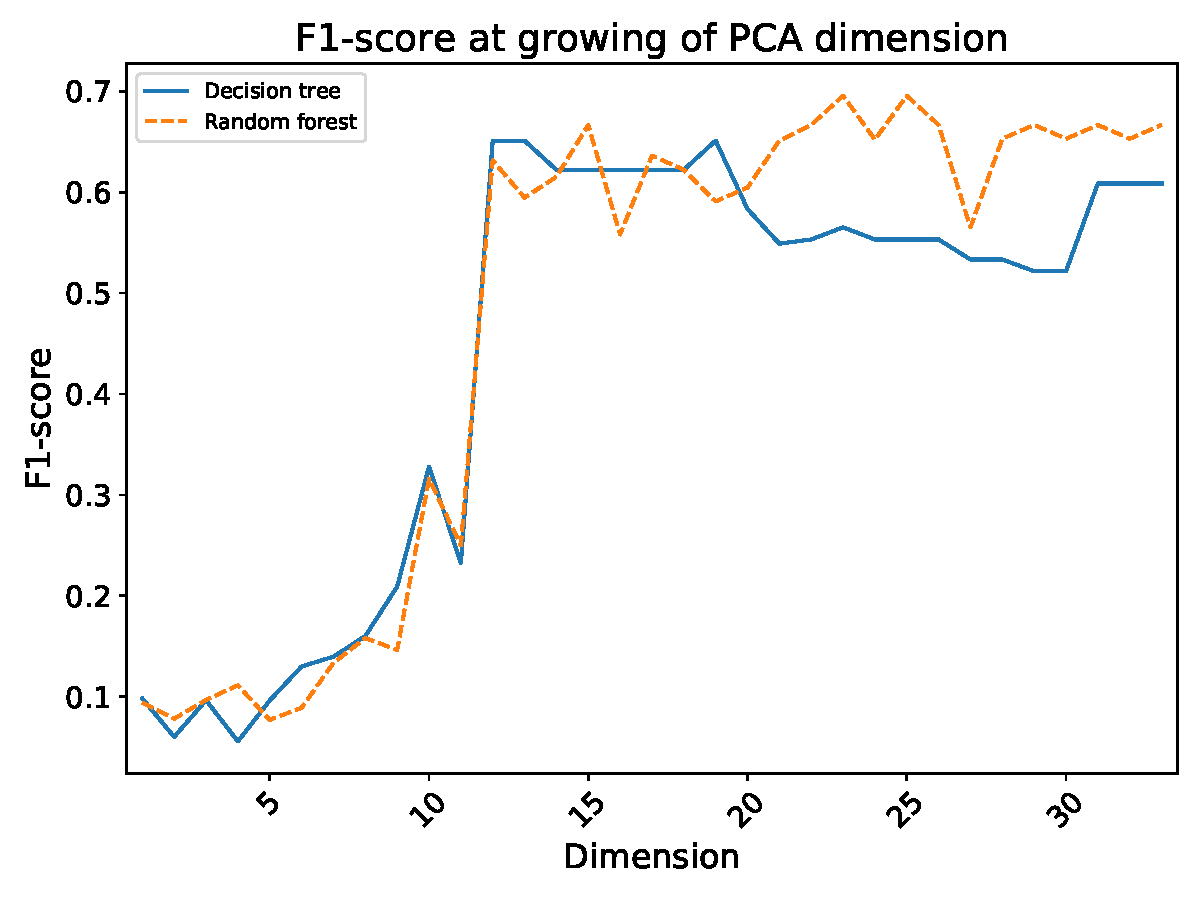
\includegraphics[width=1\linewidth]{images/pca-perf}
	\caption{Performance ottenute dai due modelli analizzati al crescere del numero di componenti della PCA utilizzate.}
	\label{fig:pca-perf}
\end{figure}
La medesima analisi è stata effettuata sul grafico riportato in Figure \ref{fig:corr-perf} relativo ai risultati dei due modelli al variare del threshold di correlazione utilizzato nella feature selection. Sorprendentemente, la soglia corrispondente a valori ottimali è estremamente bassa, pari a $0.15$; questo valore porta alla rimozione di quasi tutte le feature del dataset, mantenendo solo 5 feature. Questo risultato porta a pensare che le feature del dataset siano fortemente correlate tra loro, costituendo in larga parte informazione ridondante. Anche in questo caso, come nel precedente, l'aggiunta di feature ulteriori sembra "distrarre" il classificatore, provocando un deterioramento delle performance significativo, salvo poi recuperare avvicinandosi alla situazione del dataset completo.
\begin{figure}
	\centering
	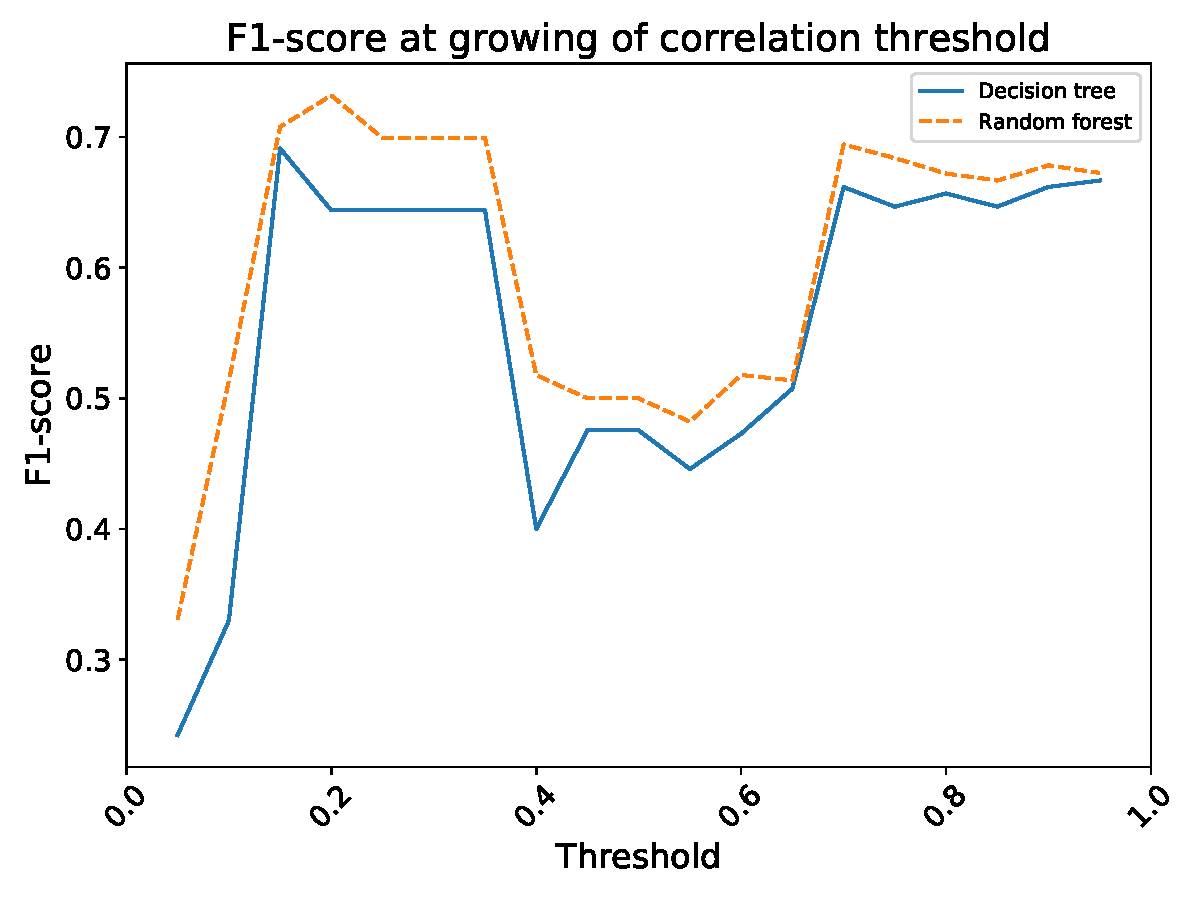
\includegraphics[width=1\linewidth]{images/corr-perf}
	\caption{Performance ottenute dai due modelli analizzati al crescere del valore di threshold del filtro di correlazione. Si noti che al crescere del valore di threshold, il numero di feature utilizzate cresce a sua volta.}
	\label{fig:corr-perf}
\end{figure}

Stabiliti quali fossero i parametri ottimali per le tecniche di \textit{feature reduction}, i vari algoritmi sono stati addestrati sui vari dataset prodotti. In particolare, per ogni input sono state testate sia alberi di decisione che random forest. Nel processo di train è stato deciso di utilizzare la tecnica di \textit{oversampling} in quanto i risultati di alcuni test preliminari effettuati hanno mostrato come l'utilizzo di tale approccio sia in grado di garantire in alcuni casi performance migliori rispetto alla versione non alterata del dataset. 
Nei casi restanti SMOTE è risultato semplicemente inefficace, senza indurre un peggioramento delle performance predittive.
\begin{table}
	\centering
	\caption{Performance medie del processo di 5-fold \textit{stratified cross-validation} sul dataset completo e dopo FR dei modelli analizzati.}
	\label{tab:f1score}
	\begin{tabular}{|c|c|c|}
		\toprule
		Modello & Tecnica da FR & f1-\textit{measure} media \\ 
		\midrule 
		Decision Tree & / & $0.647$ \\
		Random Forest & / & $0.715$ \\ 
		Decision Tree & Filtro correlazione & $0.607$ \\ 
		Random Forest & Filtro correlazione & $0.727$ \\ 
		Decision Tree & PCA & $0.691$ \\ 
		Random Forest & PCA & $0.74$ \\ 
		\bottomrule
	\end{tabular}
\end{table}
I risultati dei processi di SCV sono riportati in maniera analitica in Tabella \ref{tab:f1score} e nella Figura \ref{fig:fscore}, dalla quale è possibile notare come le performance medie dei modelli derivanti dalle random forest risultino essere migliori rispetto a quelli derivanti dagli alberi di decisione. Allo stesso modo è possibile notare come le performance medie migliori siano ottenete dal filtro delle feature basato sulla correlazione, mentre PCA e il dataset completo mostrano performance inferiori. 
\begin{figure}
	\centering
	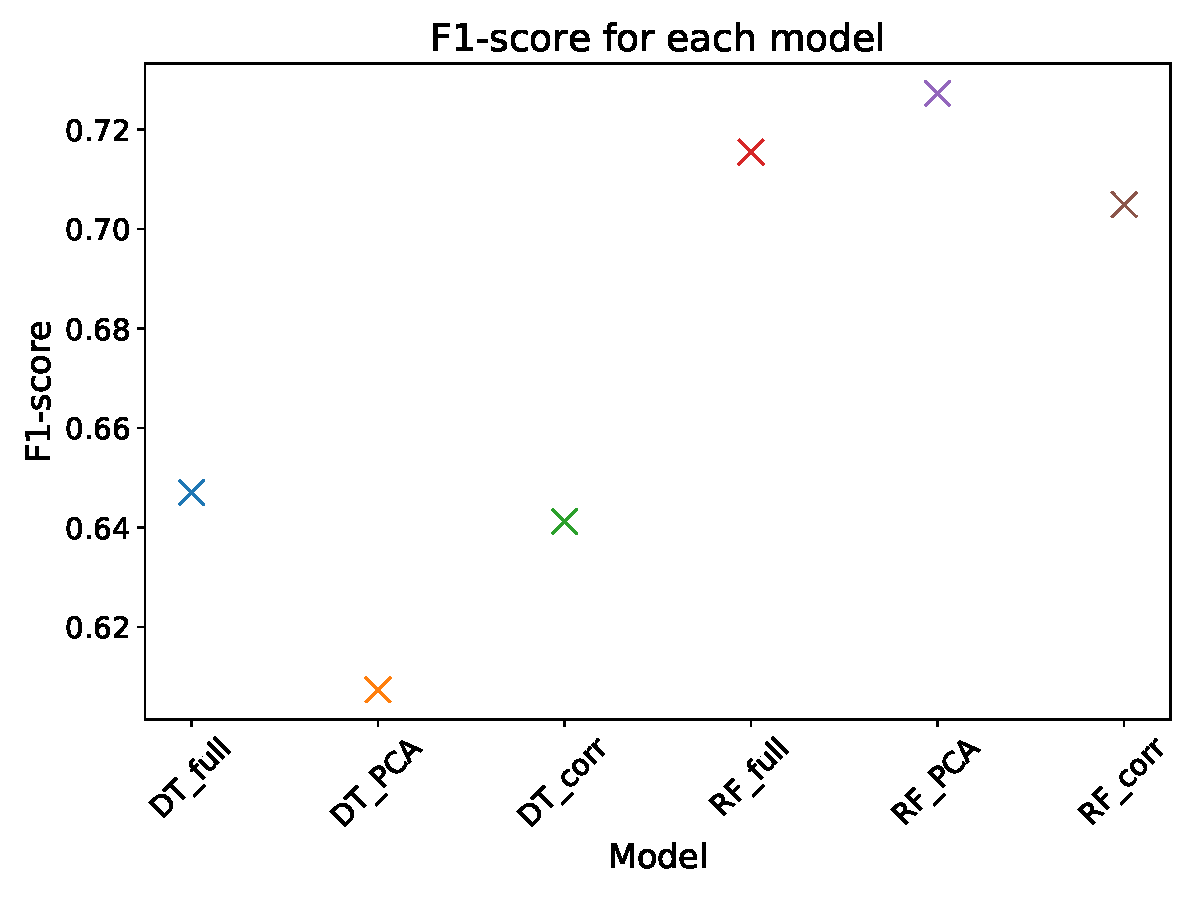
\includegraphics[width=1\linewidth]{images/fscore}
	\caption{Performance medie del processo di 5-fold \textit{stratified cross-validation} sul dataset completo e dopo FR dei modelli analizzati.}
	\label{fig:fscore}
\end{figure}
Al fine di stabilire se le differenze tra i vari modelli fossero statisticamente significative, è stato deciso di effettuare una serie di \textit{paired t-test} sulle performance dei vari modelli proposti nei differenti fold della SCV.
Analizzando in modo qualitativo i risultati associati ad ogni fold, è stata rilevata una forte eterogeneità nelle performance di ogni modello all'interno dei vari fold; un esempio di quanto affermato è riportato in Tabella \ref{tab:f1fold}, dove è possibile constatare come il range delle performance vari di oltre $20$ punti percentuali tra un fold e l'altro. Questo comportamento è probabilmente dovuto all'esiguo numero di sample disponibili, soprattutto in fase di test: l'errore di predizione su pochi sample può provocare una drastica variazione della misura di performance considerata. Pur aumentando in maniera artificiale il numero di sample della classe minoritaria nel train set, i sample sintetici risulteranno molto simili a quelli già presenti nel train set e, se essi non sono una fedele rappresentazione della distribuzione reale dei dati a causa del numero limitato di sample a disposizione, l'algoritmo di apprendimento automatico non sarà in grado di generalizzare correttamente. 
\begin{table}
	\centering
	\caption{Performance ottenute da random forest e albero di decisione con l'intero dataset in input nei vari fold della SCV.}
	\label{tab:f1fold}
	\begin{tabular}{|c|c|c|}
		\hline 
		Fold & f1-\textit{measure} RF & f1-\textit{measure} DT \\ 
		\hline 
		$1$ & $0.615$  & $0.571$\\ 
		\hline 
		$2$ & $0.846$ & $0.643$\\ 
		\hline 
		$3$ & $0.636$ & $0.615$\\ 
		\hline 
		$4$ & $0.692$ & $0.692$\\ 
		\hline 
		$5$ & $0.783$ & $0.714$\\ 
		\hline 
	\end{tabular} 
\end{table}
A conferma di quanto osservato, i test statistici non hanno evidenziato una differenza statisticamente rilevante tra le performance medie dei modelli DT e RF con input l'intero dataset e la riduzione tramite PCA. Al contrario, è emersa una differenza statisticamente rilevante tra le performance medie di alberi di decisione e random forset con input selezionato mediante correlazione. In questo caso, infatti, le RF mostrano performance statisticamente superiori agli alberi di decisione, come confermato dal test.
Lo studio è proseguito confrontando tra loro i modelli con input differenti; considerando i risultati dei test statistici appena presentati, è stato deciso di selezionare arbitrariamente le foreste per l'intero dataset e per la PCA (sarebbero stati allo stesso modo validi gli alberi di decisione, visto che non hanno mostrato performance medie statisticamente differenti), mentre per la tecnica di riduzione mediante correlazione è stata scelta la random forest in quanto mostrava performance migliori rispetto al corrispettivo albero di decisione. I risultati dei \textit{paired} t-test hanno mostrato nuovamente come non vi sia differenza statisticamente rilevante tra le performance medie dei modelli confrontati.
Un'ultima analisi realizzata in questo lavoro è stata come la rimozione delle feature relative agli esami clinici effettuati sulle pazienti potesse inficiare le performance predittive degli algoritmi di predizione considerati. 
I risultati, riportati in Tabella \ref{tab:noexamsscore}, mostrano un drastico peggioramento delle performance predittive; ciò suggerisce che l'esecuzioni di questi esami (o di alcuni di essi) sia imprescindibile al fine di un corretto riconoscimento dei pazienti affetti dal cancro alla cervice da parte del modello. 
Risulta altresì improbabile la corretta classificazione di un paziente a partire unicamente dai relativi dati dell'anamnesi.
I risultati sono di particolare interesse se incrociati con quelli ottenuti nella fase di ricerca del threshold per il filtro basato sulla correlazione. In quello studio, il valore soglia proposto risultava molto basso, portando all'utilizzo di sole 5 feature che erano però in grado di garantire performance ottimali dei modelli. Tra di esse risulta presente la feature \textit{Schiller}, che viene invece rimosso nel test appena proposto, in cui le performance risultano pesantemente degradate. Possiamo quindi supporre che questa analisi porti con se una grande quantità di informazione; per questo motivo, nel caso in cui non fosse possibile eseguire tutti gli esami clinici proposti per motivi economici o tecnici, l'esecuzione del test di Schiller garantirebbe un sostanziale incremento delle performance del modello, portando così a predizioni più accurate.
Nonostante ciò, per quanto concerne i costi bisogna considerare che il test di Schiller avviene durante l'esecuzione della colposcopia, il cui esito è un'altra delle feature considerate.
\begin{table}
	\centering
	\caption{Performance medie del processo di \textit{stratified 5-fold cross-validation} dei modelli senza considerare le feature relative ad esami strumentali effettuati sulle pazienti.}
	\label{tab:noexamsscore}
	\begin{tabular}{|c|c|}
		\toprule
		Modello & f1-\textit{measure} media \\ 
		\midrule 
		Decision Tree & $0.201$ \\
		Random Forest & $0.165$ \\ 
		\bottomrule
	\end{tabular}
\end{table}